\documentclass[11pt,a4paper]{article}
\usepackage[margin=1in]{geometry}% Tweak page margins
\usepackage{graphicx} % Required for inserting images
\usepackage{float} % Positioning of figures
\usepackage{xcolor}
\usepackage{tikz-cd}
%\usepackage{tikz-cd}
\usepackage[most]{tcolorbox}
\usepackage[outputdir=../]{minted}
\usepackage{biblatex}
%\bibliography{ref}
\usepackage{hyperref}
\usepackage{verbatim}
\usepackage{forest}



\definecolor{folderbg}{RGB}{124,166,198}
\definecolor{folderborder}{RGB}{110,144,169}

\def\Size{4pt}
\tikzset{
  folder/.pic={
    \filldraw[draw=folderborder,top color=folderbg!50,bottom color=folderbg]
      (-1.05*\Size,0.2\Size+5pt) rectangle ++(.75*\Size,-0.2\Size-5pt);  
    \filldraw[draw=folderborder,top color=folderbg!50,bottom color=folderbg]
      (-1.15*\Size,-\Size) rectangle (1.15*\Size,\Size);
  }
}


\title{Molecular programming with \textit{CRN++}, a 02257 project}
\author{
    Hans Henrik Hermansen s194042\\
    Jonathan S. Højlev s194684\\
    Rani Ey. í Bø s194067}
\date{26/06 2024}

\begin{document}
\pagenumbering{gobble}

\maketitle
\section{Abstract}
This report does clever things. 


\newpage

\pagenumbering{arabic}

\section{An interpreter for CRN++}

In the article \textit{CRN++: Molecular Programming Language}, Marko Vasic, David Soloveichik, and Sarfraz Khurshid define a language for programming chemical reactions to perform computation. They define a context-free grammar for this language and explain some of the limitations of the uses and expressiveness of the language when real-world chemical reactions enter the equation. 


\subsection{Grammar}

Looking at the grammar defined by the article in their listing 1.1, there are immediately some changes we would like to make. Besides this, we impose a few syntactic restrictions to ensure all parsed programs behave as expected. 

In the following, our changes to the grammar is listed. 




As stated in the article, the \texttt{ConcS} represents the starting concentration of the species. Thus a \texttt{conc['$\langle \text{A} \rangle$', '$\langle \text{64} \rangle$']} on line 32, effects the the concentration of \texttt{A} on line 16. We deemed this non-intuitive, and to force the concentrations to be stated at the top of the program. This was done by changing the \texttt{RootList}:
\begin{tabbing}
    $\langle \text{Crn} \rangle$ \,::=\; \= \texttt{crn= \{'$\langle \text{ConcList} \rangle$' ',' $\langle \text{StepList} \rangle$}\} \\
    
    $\langle \text{ConcList} \rangle$ \,::=\;  $ \epsilon$ \\
    
     \>\textbar \, $\langle \text{Conc} \rangle$ ',' $\langle \text{ConcList} \rangle$ \\

      $\langle \text{StepList} \rangle$ \,::=\;  $\langle \text{Step} \rangle$ \\

      \>\textbar \, $\langle \text{Step} \rangle$ ',' $\langle \text{StepList} \rangle$ \\
\end{tabbing}
Furthermore, in \texttt{CommandS} \texttt{ArithmeticS} is mentioned but not defined. We assume that it refers to the defined but not mentioned \texttt{ModuleS}, which would make much sense now that \texttt{ModuleS} contains arithmetic expressions. Therefore, we rename \texttt{ArithmeticS} to \texttt{ModuleS}.\\

Other than \texttt{ConcS}, there are also other restrictions, all of which we found easier to implement using syntactic restrictions. Firstly, all \texttt{number} must be non-negative, since chemical concentrations are always positive. Furthermore, to ensure fast and deterministic convergence of all ODEs, there can not be any cycles where one species depends on itself nor can a species be written to twice in one step. This implicitly disallows multiple \texttt{cmp} now that all \texttt{cmp} write to the same flags. Lastly, we enforce that all \texttt{ConditionalS} in a step must be mutually exclusive, e.g. \texttt{ifLT} cannot be used together with \texttt{ifLE} since both can be true simultaneously and that there can not be any nested \texttt{if}. This does not reduce expressiveness and makes it simpler to check the restrictions.



\subsection{Abstract syntax tree (AST)}
The AST is rooted in Root: 
\begin{minted}{haskell}
    type Root = R of Conc List * Step List
\end{minted}
Which forces all the \texttt{Concs} to come before the steps, where Conc is defined as:
\begin{minted}{haskell}
    type Conc = C of species * float
\end{minted}
This is then followed by all the \texttt{Steps}:
\begin{minted}{haskell}
    type Step = S of Command List
\end{minted}
Where the definition of \texttt{Command} is:
\begin{minted}{haskell}
    type Command =
        | Ld of species * species
        | Add of species * species * species
        | Sub of species * species * species
        | Mul of species * species * species
        | Div of species * species * species
        | Sqrt of species * species
        | Cmp of species * species
        | Rx of species List * species List * float
        | IfGT of Command List
        | IfGE of Command List
        | IfEQ of Command List
        | IfLT of Command List
        | IfLE of Command List
\end{minted}
And \texttt{species} is just a string, that signifies the name of the species:
\begin{minted}{haskell}
    type species = string
\end{minted}
The tree representation of the ..... program can be seen below:
\subsection{Parser}


\subsection{Type checker}
After parsing, we have an AST, however, this AST might not follow all the rules extraneous to the grammar. By recursively matching on each \texttt{StepList} in the AST, we check all the constraints mentioned in the section on the grammar, for example, that the conditionals in a step do not overlap and that no species is written to twice. While traversing the \texttt{StepList}, a graph $G$ is built, whose nodes represent species and an edge from $a\to b$ signals that $a$ is input to $b$. By then trying to topologically sort $G$, we can quickly check if $G$ is a $DAG$ and thereby does not contain any cycles.

\subsection{State and interpreter}
The state is quite simply just a map from each species to its corresponding value:
\begin{minted}{haskell}
    type State = Map<species, float>
\end{minted}
Since each \texttt{State} only depends on the last \texttt{State} and the steps, one can make an infinite \texttt{State} sequence, by implementing a function that generates the next state based on the current state:
\begin{minted}{haskell}
    let doStep (S(cl): Step) (state: State) : State = doCommandList cl state
\end{minted}
and utilizing it in an unfold. The interoperate function then becomes:
\begin{minted}{haskell}
    let interpretProgram (R(concl, stepl)) =

        if not (isTyped (R(concl, stepl))) then
            failwith "Does not typecheck"
        else
            let initialState = getInitialState concl
    
            Seq.unfold
                (fun (state, i) ->
                    let nextState = doStep (List.item (i % List.length stepl) stepl) state
                    Some(nextState, (nextState, i + 1)))
                (initialState, 0)
\end{minted}

Where \texttt{getInitialState} just reads all the initial concentrations:
\begin{minted}{haskell}
    let getInitialState (concl: Conc List) : State =
        List.fold (fun state (C(s, c)) -> Map.add s c state) Map.empty concl
\end{minted}

\subsection{Testing}
We wanted to use property based testing, in the hope that it would be as applicable here as it was when drawing trees in the first project. However, there were some obstacles. It was not easy to get \texttt{FsCheck} to generate an AST that could have resulted from a valid parsed program. Furthermore, generating programs and then parsing them was also not doable, since the fraction of valid programs over invalid programs is vanishingly small. Thus we opted for a more traditional approach to testing, where we have programs that we know are correct and programs that we know are flawed, and we make tests on these. \texttt{FsCheck} then picks one of these programs and we check that mapping shuffle on each \texttt{StepList} does not change whether it type checks or the resulting sequence of states. Since one cannot compare infinite sequences directly, we only check whether the first 50 steps match.\\

To increase the coverage of the tests, the individual arithmetic operators were tested in isolation, where \texttt{FsCheck} picks for example the numbers to add. These were then compared to the result from the arithmetic operations in \texttt{F\#}.

\subsection{Visualization}
To visualize the sequence of states, we first output the sequence to a file, in a manner where we can easily read it into Python.

We then load this into Python and get a list of all the species, and a matrix where row $i$ corresponds to the concentration in step $i$. The $j$th index in all rows refers to the concentration of the $j$th species, therefore, by transposing the matrix, the $i$th row becomes the data points that are to be plotted for species $i$. By then having two copies of each value except the last value, and having the x-axis $0,0.99,1,1.99,2,2.99\dots$ instead of $0,1,2\dots$ we get the stair plot that clearly shows the step-wise process instead of a continuous progression between steps.

To make the plot a bit nicer and easier to read, the lines have different opaque colours and one can elect which species are plotted through command line arguments. An example is shown in the following figure:
\begin{figure}[H]
    \centering
    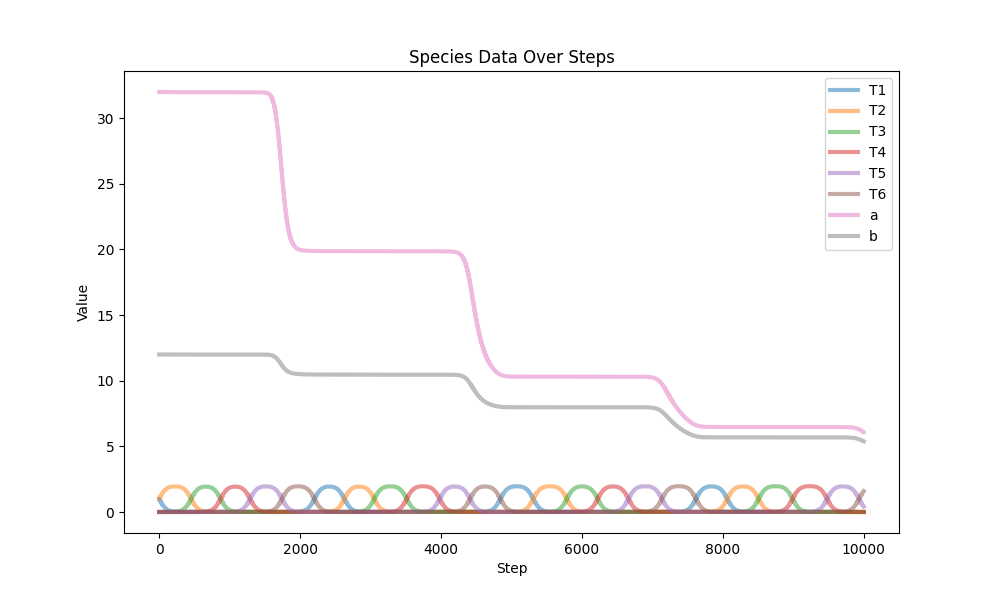
\includegraphics[scale=0.4]{report/figures/examplePlot.png}
    %\caption{Caption}
    %\label{fig:enter-label}
\end{figure}

\subsection{Assessment}
\section{Chemical reactions}

\subsection{Reactions and CRN}
A reaction is a set of reactants, a set of products, and a number $\kappa$ representing the speed of the reaction. Each reactant and product is some quantity of a species which can be modelled as:  
\begin{minted}{haskell}
    type Reaction = Rxn of Map<species, float> * Map<species, float> * float
\end{minted}
Where the maps map a species to its concentration, the first map is the reactants, the second map is the products and the final float is $\kappa$.

Then \texttt{CRN} can be defined as the union of all the reactions, which can be stored in a reaction list:
\begin{minted}{haskell}
    type CRN = Reaction List
\end{minted}

\subsection{Parser}

For chemical reactions we did actually implement a parser that can parse a string of chemical reactions. However we did not ever use it as the as our compiler takes an AST and compiles it directly to a list of our \texttt{F\#} type \texttt{Rxn(r,p,c)}. Therefore there is no need for a parser for the reactions. % The grammer for the parser can be seen in the appendix

\subsection{Simulation}
The system of ODE's that we want to simulate describes the rate of change of concentration for a species \( S \) within a CRN. The equation is:
\begin{equation}\label{eq:diff}
    \frac{d[S]}{dt} = \sum_{\forall \text{rxn} \in \text{CRN}} \kappa(\text{rxn}) \cdot \text{netChange}(S,\text{rxn}) \cdot \prod_{\forall R \in \text{reactants}(\text{rxn})} [R]^{m_{\text{rxn}}(R)}(t)
\end{equation}

This can be broken down into its components and translated to code. The most important part is of course that the simulation is a discretization of the continuous system. Here, $\frac{dS}{dt}$ is replaced by $\frac{\Delta S}{\Delta t}$ and $\Delta t$ is moved to the other side of the equation. The resulting equation can then be reformulated to use matrix operations, which in practice are highly optimized:

\[
\Delta \mathbf{S}(t) = \mathbf{N} \cdot \mathbf{v}(t)
\]
Where:
\begin{itemize}
    \item \( \mathbf{N} \) is the net change matrix, and each element \( \mathbf{N}_{ij} \) represents the scaled net change in species \( i \) due to reaction \( j \), including the reaction rate \( \kappa \). 
% \begin{minted}{haskell}
% let genNetChangeMatrix (crn : CRN) (sl : species List) = 
%     Matrix.ofJaggedList (List.foldBack (fun s st -> 
%         genNetChangeList crn s :: st) sl [])
% \end{minted}
%Where \texttt{genNetChangeList} multiplies the reaction speed $c$ with the \texttt{netChange}:
% \begin{minted}{haskell}
%     let genNetChangeList (crn : CRN) (s : species) = 
%         (List.foldBack (fun (Rxn(r,p,c)) st -> 
%             c * (calcNetChange (Rxn(r,p,c)) s) :: st) crn [])
% \end{minted}
%and the \texttt{netChange} is calculated by:
% \begin{minted}{haskell}
%     let calcNetChange (Rxn(r, p, c)) (s: species) = 
%         (getValue p s) - (getValue r s) 

% \end{minted}

    \item \( \mathbf{v}(t) \) is a vector where each component corresponds to the product of the concentrations of reactants raised to their stoichiometric coefficients for each reaction at time \( t \). This vector depends on $S(t)$ and is therefore calculated at each time step. It plays the same role as the product in equation \ref{eq:diff}. 
    %This vector is computed by:
% \begin{minted}{haskell}
% let calcReactionProducts (state : State) (crn : CRN) = 
%     vector (
%         List.map (fun (Rxn(r, _, _)) ->
%             Map.fold (fun s coeff prod -> 
%                 prod * (state |> Map.find s) ** coeff) 1.0 r
%         ) crn
%     )
% \end{minted}
    \item $\Delta \mathbf{S}$ is a vector containing the change for each species at some time. This vector is added to the current State which yields the simulated state at time $t+\Delta t$. 
    %This is calculated in the following way
    %     \begin{minted}{haskell}
    %     let calcDerivatives netChangeMatrix reactionProduct timestep =
    %         timestep * (netChangeMatrix * reactionProduct) 
    % \end{minted}
\end{itemize}

We wanted to further optimize the calculation of \(\mathbf{v}(t)\), by using the logarithm to transform it into a dot-product, however this led to problems since it is possible for concentrations to be zero. In summary, the updated state can be calculated by transforming the current state to the $\mathbf{v}$ vector and performing a dot product with a constant matrix defined in preprocessing. Lastly, the infinite sequence of states can then be calculated using a \texttt{Seq.unfold} similar to the code for the interpreter, using the function for updating a state to the next. See the code for more details. 

\subsection{Visualization}
Since this simulation results in a sequence of states, just like the interpreter from the prior section, we can use the visualization code from the interpreter to visualize the simulation. The plots for this section can be seen in appendix \ref{sec:compiler_plots}.

\subsection{Testing}
As with the interpreter, all the modules from Table 1 in the paper were tested individually for the simulator. All of them passed all tests, except the \texttt{cmp} and \texttt{sub} modules. For \texttt{cmp} we encountered for some values that the binary flags \texttt{Xegty} among the other, have problems reaching 0 and 1. For \texttt{sub} we encountered some of the problems also described in the article. The \texttt{sub} module is by far the module with highest error and when \texttt{X} is very close to or equal to \texttt{Y} in \texttt{X-Y} the error becomes very high. This however is expected so there is really no reason to try and fix this. More on this in the assessment.

\subsection{Assessment}
As a whole, we are pleased with the outcome of this section. The optimization of the simulation using matrix operations was especially rewarding. The tests also proved helpful, both for finding and fixing bugs, but also for figuring out that the simulation of the \texttt{cmp} module does not behave as expected. When simulating \texttt{cmp}, for example \texttt{cmp[a,b]}, the error becomes larger as the fraction $\frac{a}{b}$ goes to 1. Even if we make the requirements easier, \texttt{cmp} will still fail given two large enough neighbouring numbers. This is illustrated in the following figure:
\begin{figure}[H]
    \centering
    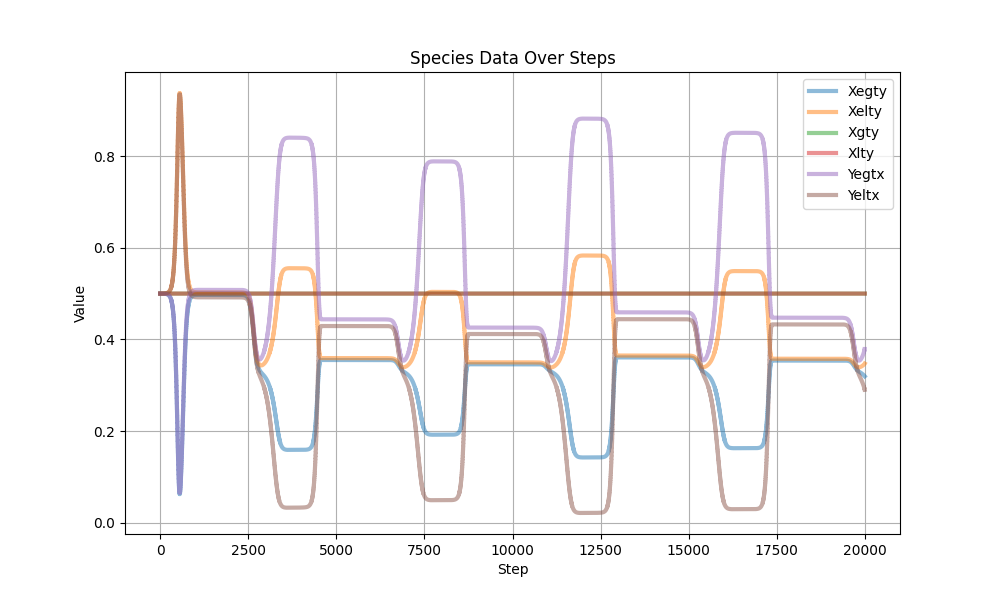
\includegraphics[scale=0.22]{report/figures/cmpbad.png}
    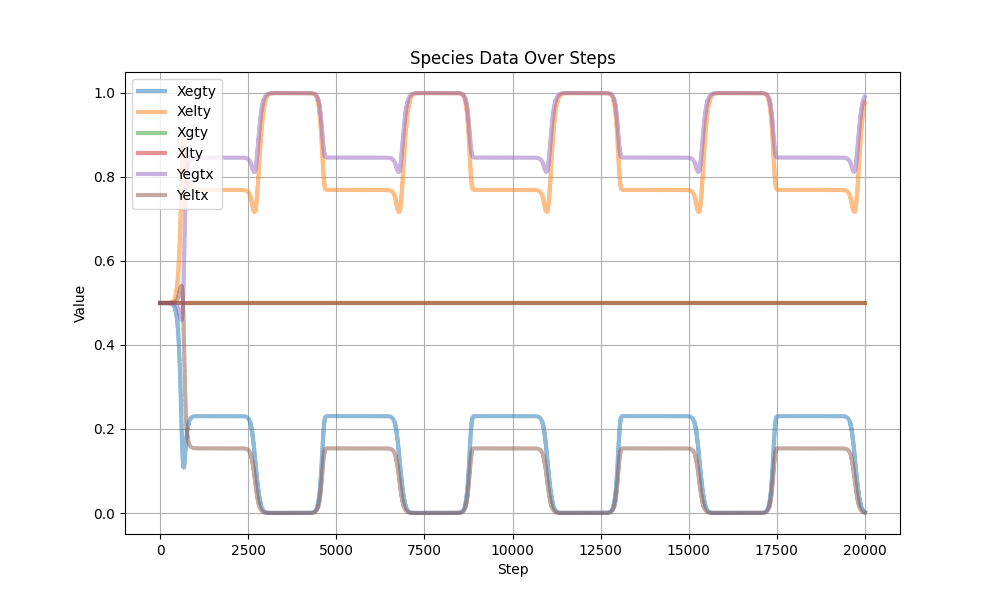
\includegraphics[scale=0.22]{report/figures/cmpgood.png}
    \caption{Plot of compare, where the right one does well on the numbers 1 and 5, while the left one does a bit poorer on 45 and 46.}
\end{figure}

The only negative part was that we never had a reason to use the parser for chemical reactions (point 9), which led to it feeling less rewarding and more like only an obligation.

\section{Compiling CRN++ to chemical reactions}


\section{Evaluation}

This project on CRN++ implementation gave us a hands-on opportunity to deepen our understanding of the F\# programming language while diving into the intriguing world of chemical computation. We successfully enhanced the grammar and integrated matrix operations for more efficient ODE solutions, making our simulations significantly faster. These improvements allowed us to handle larger cases and in combination with our visualization tools, it offered clearer insights into the chemical processes.

Despite these advancements, we encountered challenges, particularly in executing operations within each step correctly to mimic the intended chemical behaviours. This highlighted the importance of proper sequence execution, which we aimed to address through topological sorting in our interpreter — a goal we unfortunately ran out of time to fully implement. 


\newpage
\section{Appendix}
\pagenumbering{roman}

\subsection{Structure}

\subsection{Assessment of structure}



\subsection{Figure 5 from the paper}


\subsection{Pathological case from the paper}




%\printbibliography

\end{document}
